\usetikzlibrary{arrows.meta,calc}
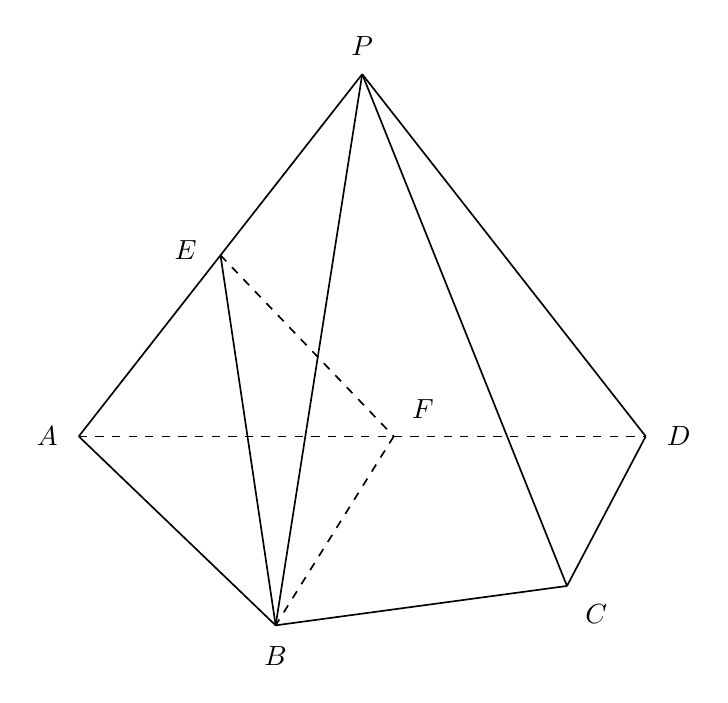
\begin{tikzpicture}[x=1cm,y=1cm,font=\normalsize,line width=.6pt]
\coordinate (P) at (0,4.6);
\coordinate (A) at (-3.6,0);
\coordinate (D) at (3.6,0);
\coordinate (F) at (0.4,0);
\coordinate (B) at (-1.1,-2.4);
\coordinate (C) at (2.6,-1.9);
\coordinate (E) at (-1.8,2.3);
% base outline: front edges solid, back edge AD dashed
\draw[solid] (A) -- (B) -- (C);
\draw[solid] (C) -- (D);
% base hidden edge A-D split at F
\draw[dashed] (A) -- (F);
\draw[dashed] (F) -- (D);
% lateral edges from apex
\draw[solid] (P) -- (A);
\draw[solid] (P) -- (B);
\draw[solid] (P) -- (C);
\draw[solid] (P) -- (D);
% auxiliary segments
\draw[solid] (E) -- (B);
\draw[dashed] (E) -- (F);
\draw[dashed] (F) -- (B);
% labels with clearance
\node[above,yshift=3pt] at (P) {$P$};
\node[left,xshift=-4pt] at (A) {$A$};
\node[right,xshift=4pt] at (D) {$D$};
\node[below,yshift=-4pt] at (B) {$B$};
\node[below right,xshift=3pt,yshift=-3pt] at (C) {$C$};
\node[left,xshift=-5pt,yshift=2pt] at (E) {$E$};
\node[above right,xshift=3pt,yshift=3pt] at (F) {$F$};
\end{tikzpicture}
